%! Author = yanni
%! Date = 18.10.2021

\documentclass[a4paper,12pt]{article}
\usepackage{fancyhdr}
\usepackage{fancyheadings}
\usepackage[ngerman,german]{babel}
\usepackage{german}
\usepackage[utf8]{inputenc}
%\usepackage[latin1]{inputenc}
\usepackage[active]{srcltx}
\usepackage{algorithm}
\usepackage[noend]{algorithmic}
\usepackage{amsmath}
\usepackage{amssymb}
\usepackage{amsthm}
\usepackage{bbm}
\usepackage{enumerate}
\usepackage{graphicx}
\usepackage{ifthen}
\usepackage{listings}
\usepackage{struktex}
\usepackage{hyperref}
\usepackage[T1]{fontenc}

%%%%%%%%%%%%%%%%%%%%%%%%%%%%%%%%%%%%%%%%%%%%%%%%%%%%%%
%%%%%%%%%%%%%% EDIT THIS PART %%%%%%%%%%%%%%%%%%%%%%%%
%%%%%%%%%%%%%%%%%%%%%%%%%%%%%%%%%%%%%%%%%%%%%%%%%%%%%%
\newcommand{\Fach}{Datenbanksysteme I}
\newcommand{\Name}{Yannick Brenning}
\newcommand{\Seminargruppe}{C}
\newcommand{\Matrikelnummer}{3732848}
\newcommand{\Semester}{WiSe 21/22}
\newcommand{\Uebungsblatt}{2} %  <-- UPDATE ME
%%%%%%%%%%%%%%%%%%%%%%%%%%%%%%%%%%%%%%%%%%%%%%%%%%%%%%
%%%%%%%%%%%%%%%%%%%%%%%%%%%%%%%%%%%%%%%%%%%%%%%%%%%%%%

\setlength{\parindent}{0em}
\topmargin -1.0cm
\oddsidemargin 0cm
\evensidemargin 0cm
\setlength{\textheight}{9.2in}
\setlength{\textwidth}{6.0in}

%%%%%%%%%%%%%%%
%% Aufgaben-COMMAND
\newcommand{\Aufgabe}[1]{
        {
        \vspace*{0.5cm}
        \textbf{Aufgabe #1}
        \vspace*{0.2cm}
    }
}
%%%%%%%%%%%%%%
\hypersetup{
    pdftitle = {\Fach{}: Übungsblatt \Uebungsblatt{}},
    pdfauthor = {\Name},
    pdfborder = {0 0 0}
}

\lstset{ %
    language=java,
    basicstyle=\footnotesize\tt,
    showtabs=false,
    tabsize=2,
    captionpos=b,
    breaklines=true,
    extendedchars=true,
    showstringspaces=false,
    flexiblecolumns=true,
}

\title{Übungsblatt \Uebungsblatt{}}
\author{\Name{}}

\begin{document}
    \thispagestyle{fancy}
    \lhead{\Fach{} \\ \small \Name{} - \Matrikelnummer{}}
    \rhead{\Semester{} \\  Übungsgruppe \Seminargruppe{}}
    \vspace*{0.2cm}
    \begin{center}
        \LARGE \textbf{Übungsblatt \Uebungsblatt{}}
    \end{center}
    \vspace*{0.2cm}

%%%%%%%%%%%%%%%%%%%%%%%%%%%%%%%%%%%%%%%%%%%%%%%%%%%%%%
%% Insert your solutions here %%%%%%%%%%%%%%%%%%%%%%%%
%%%%%%%%%%%%%%%%%%%%%%%%%%%%%%%%%%%%%%%%%%%%%%%%%%%%%%

    \Aufgabe{1:}ER-Modell \\
    \begin{enumerate}[(a)]
        \item Ein \emph{Entity} ist ein Gegenstand, der ein abstraktes oder reales Objekt der physischen Welt repräsentiert. \\
        Entities mit gleichen Eigenschaften werden zu \emph{Entity-Mengen} zusammengefasst (Klassifikation).
        \item Ein Beispiel für eine Entity wäre ein Student an einer Universität.
        Hierbei wäre die Eigenschaft \texttt{NAME[Vorname: char(30), Nachname: char(30)]} eine zusammengesetzte Eigenschaft
        von der Entität \texttt{Student}, da sie eine Kombination mehrerer Attribute ist, die zusammen hängen. \\
        Ein Beispiel für ein mehrwertiges Attribut wäre das aktuelle Semester \texttt{SEMESTER[int]},
        in dem sich der Student befindet, da sich dieses Attribut verändert und verschiedene Werte annimmt. \\
        Ein zusammengesetztes und mehrwertiges Attribut wären bspw. die Studiengänge eines Students
        \texttt{STUDIENGÄNGE[Studiengang1: char(30), Studiengang2: char(30)]}.
        \item Ein Beispiel für eine schwache Entity-Menge ist eines von mehreren Projekt-Dokumenten, welches zu
        einer Projekt-Entität gehört.
    \end{enumerate}

    \Aufgabe{2:}Schlüsselkandidaten \\
    \begin{enumerate}[(a)]
        \item Schlüsselkandidaten sind einwertige Attribute oder Attributkombinationen, die einzelne Entities einer
        Entity-Menge eindeutig identifizieren. Primärschlüssel sind Schlüsselkandidaten, die zur eindeutigen Identifizierung
        eines bestimmten Datensatzes verwendet werden.
        \item Die Matrikelnummer ist für jeden Studenten einzigartig, also wäre dieser ein optimaler Schlüsselkandidat.
    \end{enumerate}

    \Aufgabe{3:}Abbildungstypen \\
    \begin{enumerate}[(a)]
        \item
        \item
        \item Es muss jede Beziehung die Kardinalität 1 haben.
    \end{enumerate}

    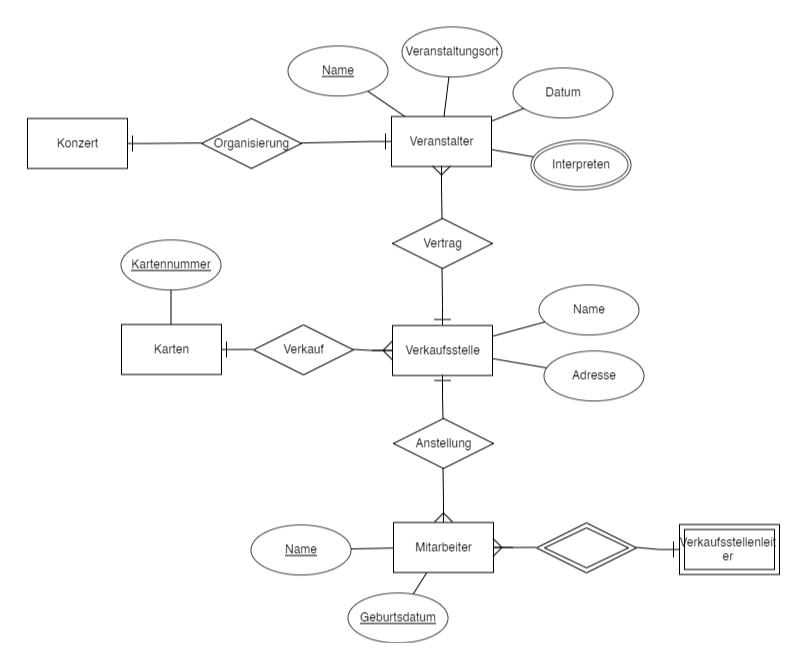
\includegraphics[width=\linewidth]{DBS-UEB02-A4.png}
    \caption{\Aufgabe{4:}ER-Modell Erstellung} \\

    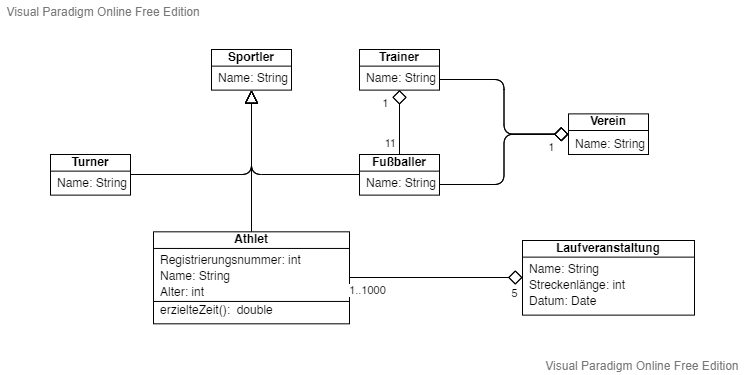
\includegraphics[width=\textwidth]{DBS-UEB02-A5.png}
    \caption{\Aufgabe{5:}UML}

%%%%%%%%%%%%%%%%%%%%%%%%%%%%%%%%%%%%%%%%%%%%%%%%%%%%%%
%%%%%%%%%%%%%%%%%%%%%%%%%%%%%%%%%%%%%%%%%%%%%%%%%%%%%%
\end{document}